\documentclass[11pt, a4paper]{article}
\usepackage{pdfpages}
\usepackage{parallel}
\usepackage[T2A]{fontenc}
%\usepackage{ucs}
\usepackage[utf8]{inputenc}
\usepackage[english,russian]{babel}
\usepackage{hyperref}
\usepackage{rotating}
\usepackage[inner=2cm,top=1.8cm,outer=2cm,bottom=2.3cm,nohead]{geometry}
%\usepackage{listings}
\usepackage{graphicx}
\usepackage{wrapfig}
\usepackage{longtable}
\usepackage{indentfirst}
\usepackage{array}
\usepackage{tikzsymbols}
\usepackage{soul}
\usepackage[ruled,vlined]{algorithm2e}
\usepackage{qrcode}
\counterwithout{figure}{section} 

\usepackage{url}
\makeatletter
\g@addto@macro{\UrlBreaks}{\UrlOrds}
\makeatother

\newcolumntype{P}[1]{>{\raggedright\arraybackslash}p{#1}}
\frenchspacing
%\usepackage{fixltx2e} %text sub- and superscripts
\usepackage{icomma} % коскі ў матэматычным рэжыме
%\PreloadUnicodePage{4}

\newcommand{\longpage}{\enlargethispage{\baselineskip}}
\newcommand{\shortpage}{\enlargethispage{-\baselineskip}}

\def\switchlang#1{\expandafter\csname switchlang#1\endcsname}
\def\switchlangbe{
\let\saverefname=\refname%
\def\refname{Літаратура}%
\def\figurename{Іл.}%
}
\def\switchlangru{
\let\saverefname=\refname%
\let\savefigurename=\figurename%
\def\refname{Литература}%
\def\figurename{Рис.}%
}
\def\switchlangen{
\let\saverefname=\refname%
\def\refname{References}%
\def\figurename{Fig.}%
}

\hyphenation{admi-ni-stra-tive}
\hyphenation{ex-pe-ri-ence}
\hyphenation{fle-xi-bi-li-ty}
\hyphenation{Py-thon}
\hyphenation{ma-the-ma-ti-cal}
\hyphenation{re-ported}
\hyphenation{imp-le-menta-tions}
\hyphenation{pro-vides}
\hyphenation{en-gi-neering}
\hyphenation{com-pa-ti-bi-li-ty}
\hyphenation{im-pos-sible}
\hyphenation{desk-top}
\hyphenation{elec-tro-nic}
\hyphenation{com-pa-ny}
\hyphenation{de-ve-lop-ment}
\hyphenation{de-ve-loping}
\hyphenation{de-ve-lop}
\hyphenation{da-ta-ba-se}
\hyphenation{plat-forms}
\hyphenation{or-ga-ni-za-tion}
\hyphenation{pro-gramming}
\hyphenation{in-stru-ments}
\hyphenation{Li-nux}
\hyphenation{sour-ce}
\hyphenation{en-vi-ron-ment}
\hyphenation{Te-le-pathy}
\hyphenation{Li-nux-ov-ka}
\hyphenation{Open-BSD}
\hyphenation{Free-BSD}
\hyphenation{men-ti-on-ed}
\hyphenation{app-li-ca-tion}

\def\progref!#1!{\texttt{#1}}
\renewcommand{\arraystretch}{2} %Іначай формулы ў матрыцы зліпаюцца з лініямі
\usepackage{array}

\def\interview #1 (#2), #3, #4, #5\par{

\section[#1, #3, #4]{#1 -- #3, #4}
\def\qname{LVEE}
\def\aname{#1}
\def\q ##1\par{{\noindent \bf \qname: ##1 }\par}
\def\a{{\noindent \bf \aname: } \def\qname{L}\def\aname{#2}}
}

\def\interview* #1 (#2), #3, #4, #5\par{

\section*{#1\\{\small\rm #3, #4. #5}}
\ifx\ParallelWhichBox\undefined%
    \addcontentsline{toc}{section}{#1, #3, #4}%
\else%
\ifnum\ParallelWhichBox=0%
    \addcontentsline{toc}{section}{#1, #3, #4}%
\fi\fi%

\def\qname{LVEE}
\def\aname{#1}
\def\q ##1\par{{\noindent \bf \qname: ##1 }\par}
\def\a{{\noindent \bf \aname: } \def\qname{L}\def\aname{#2}}
}

\newcommand{\interviewfooter}[1]{
\vskip 1em
\noindent \textit{#1}
}

\AtEndDocument{\vfill\centering \qrcode{https://github.com/fiowro/mouses/blob/main/\jobname.pdf}}

\switchlang{en}
\begin{document}

\title{1984 "--- Siemens PC-D mouse}
\date{}
\maketitle
\selectlanguage{english}
In 1984, Siemens announced the PC-D personal computer working under MS DOS but not hardware compatible with IBM PC. This computer was based on Intel 80186 processor, had proprietary monochrome graphics adapter with 12-inch display, custom keyboard, and RAM varying from 128 Kb to 1 Mb. Software included MS DOS 2.11 and Windows 1.0 as well as a number of office applications and few simple games \cite{wiki}. One year later a two-button mouse (figure \ref{fig:SiemensPCDPic}) was added to the list of its optional peripheral devices \cite{blog}.

\begin{figure}[h]
    \centering
    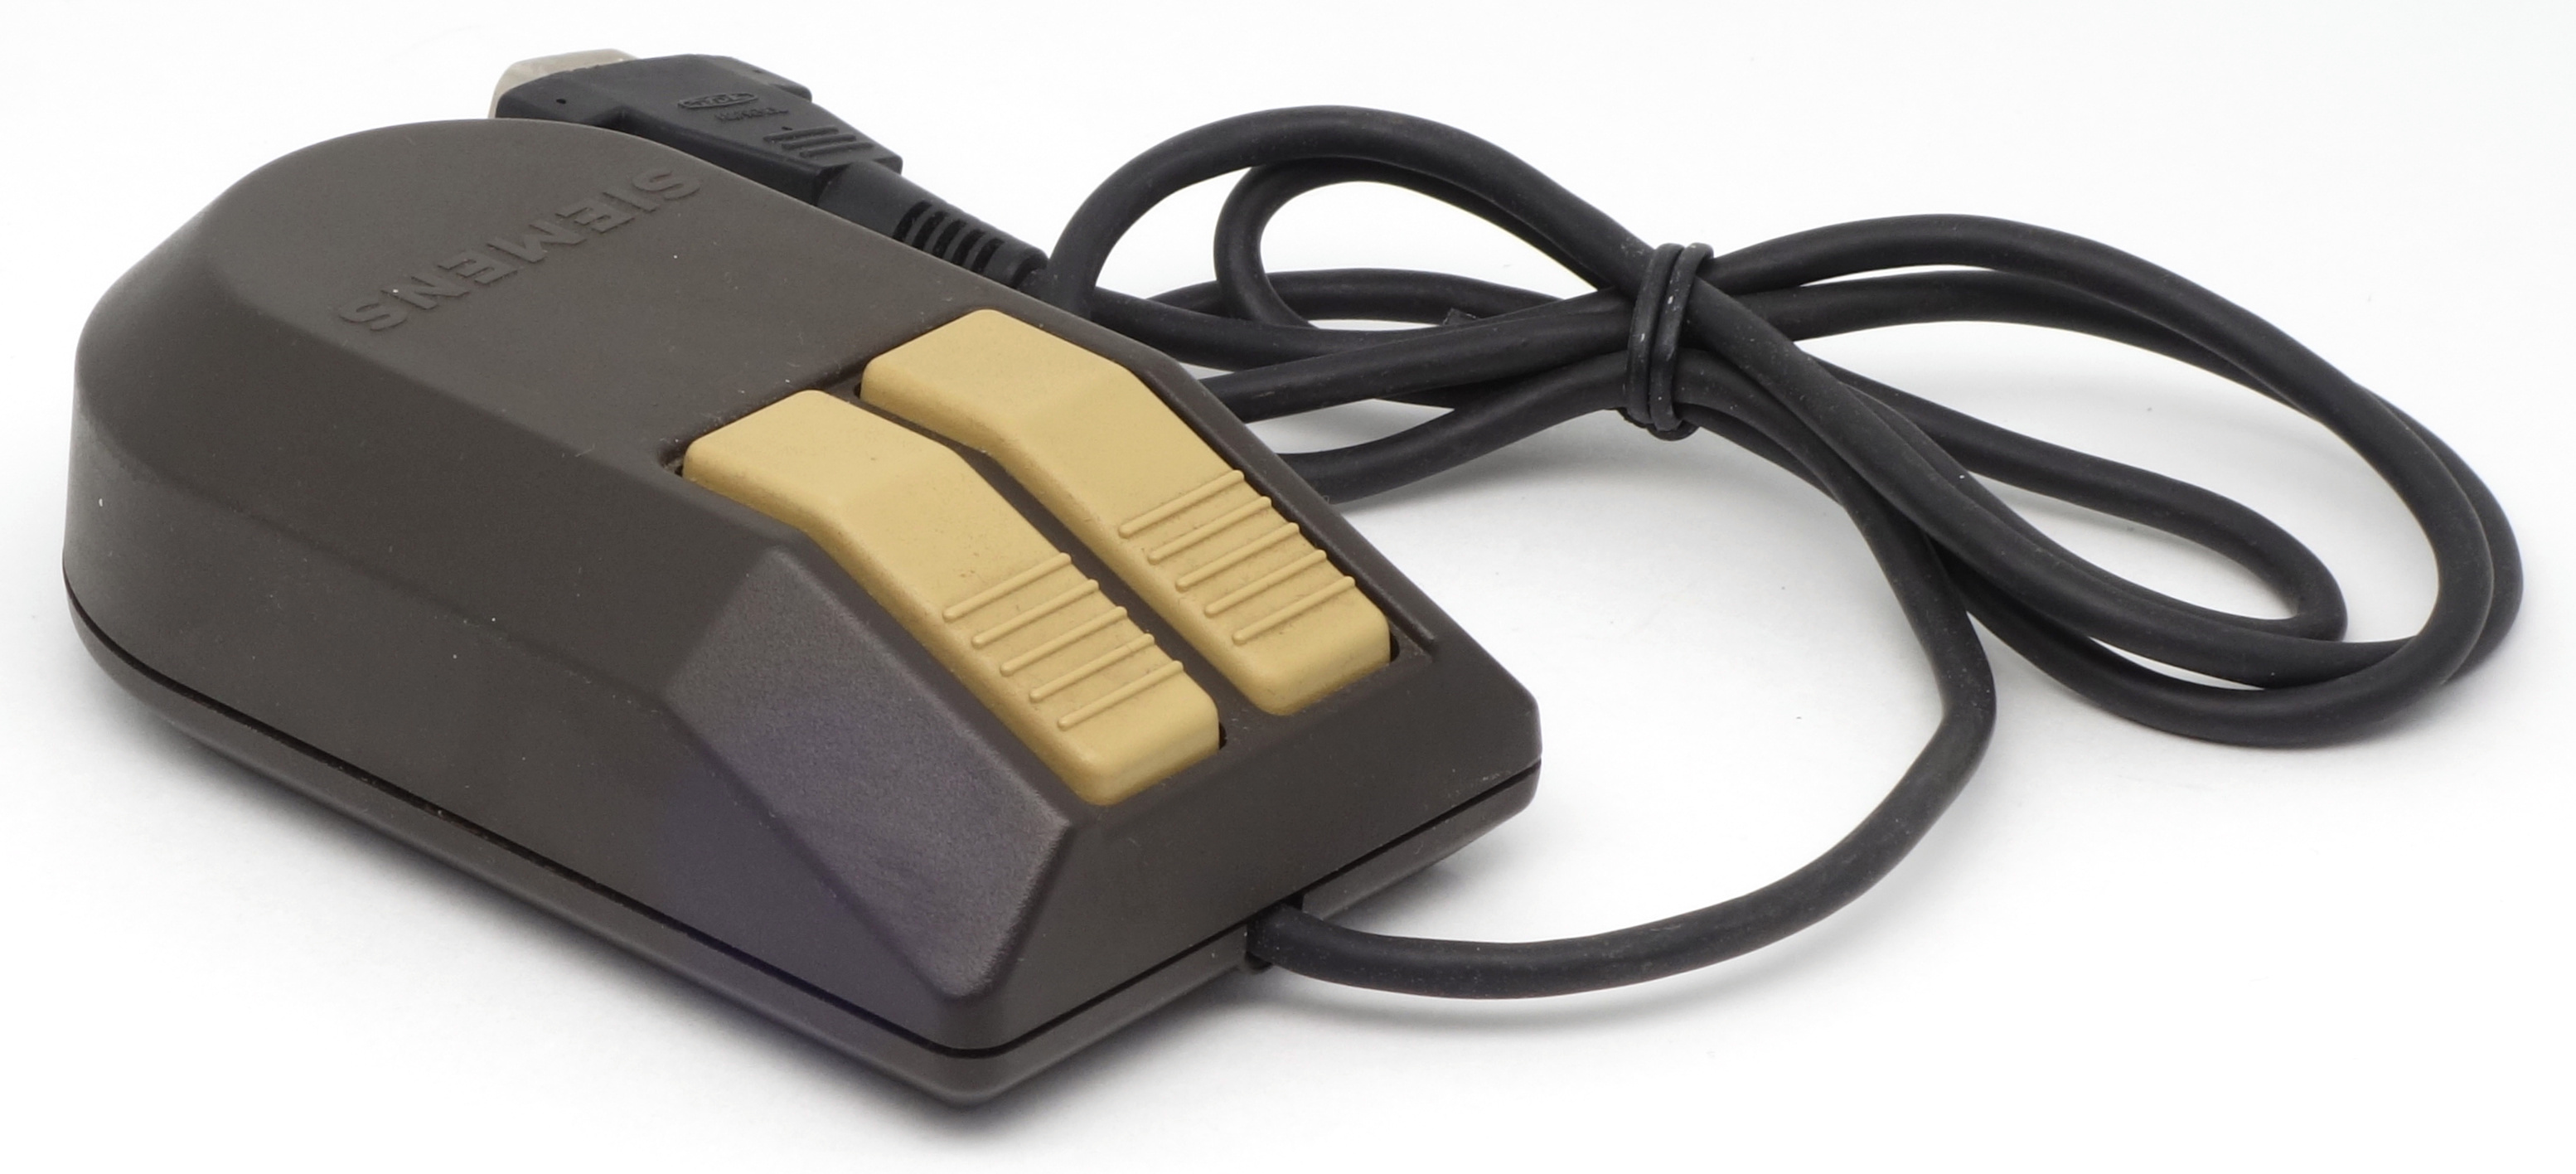
\includegraphics[scale=0.65]{1985_siemens_pcd_mouse/pic_30.jpg}
    \caption{Siemens PC-D Mouse}
    \label{fig:SiemensPCDPic}
\end{figure}

As you can see (figure \ref{fig:SiemensPCDTopBottom}), , the mouse is made in a contrasting black and beige color scheme (however, there are also photographs of this mouse in a plain beige case). On top there are two buttons with a relief pattern and the company name; in general, the body has a complex chopped shape and does not contain additional elements. The bottom contains a rubberized ball and a locking ring that can be pushed to the side to remove the ball for cleaning the mouse. Around the locking ring there is a contrasting ring-shaped pad made of low-friction material, which is a hallmark of many mice of the 80s designed in Japan.

\begin{figure}[h]
    \centering
    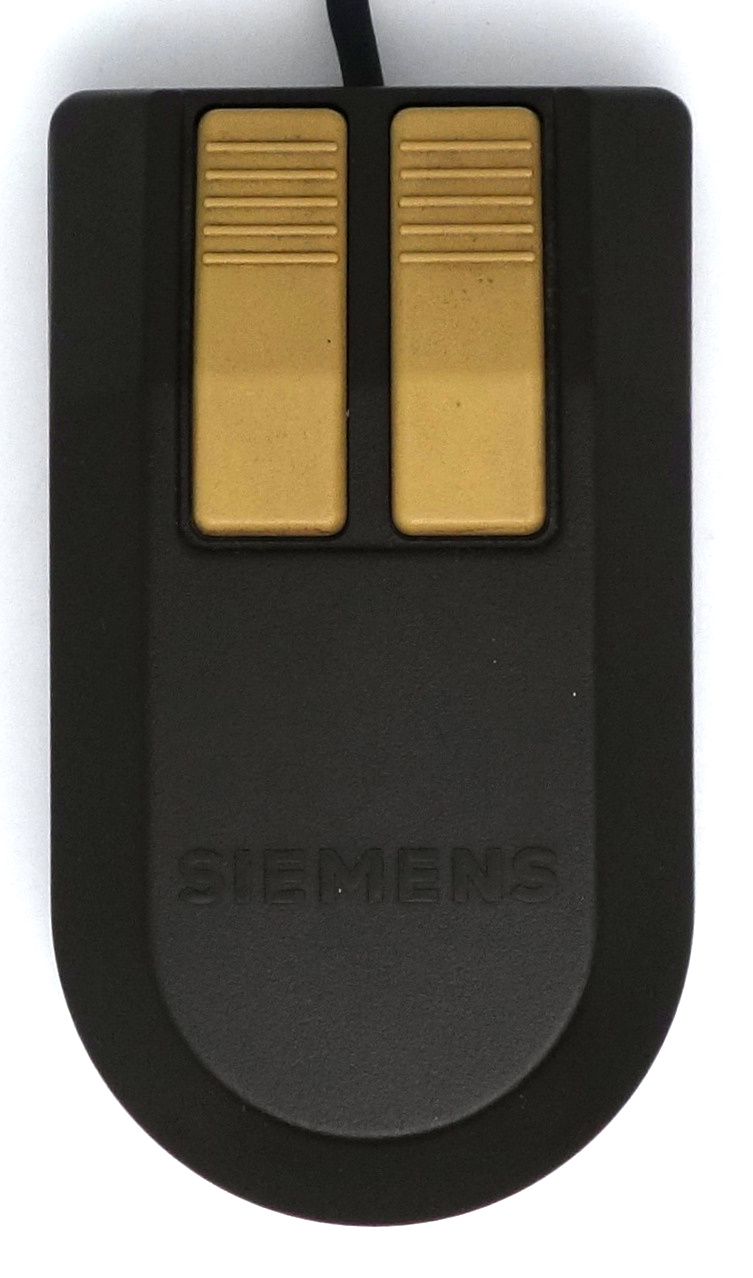
\includegraphics[scale=0.5]{1985_siemens_pcd_mouse/top_30.jpg}
    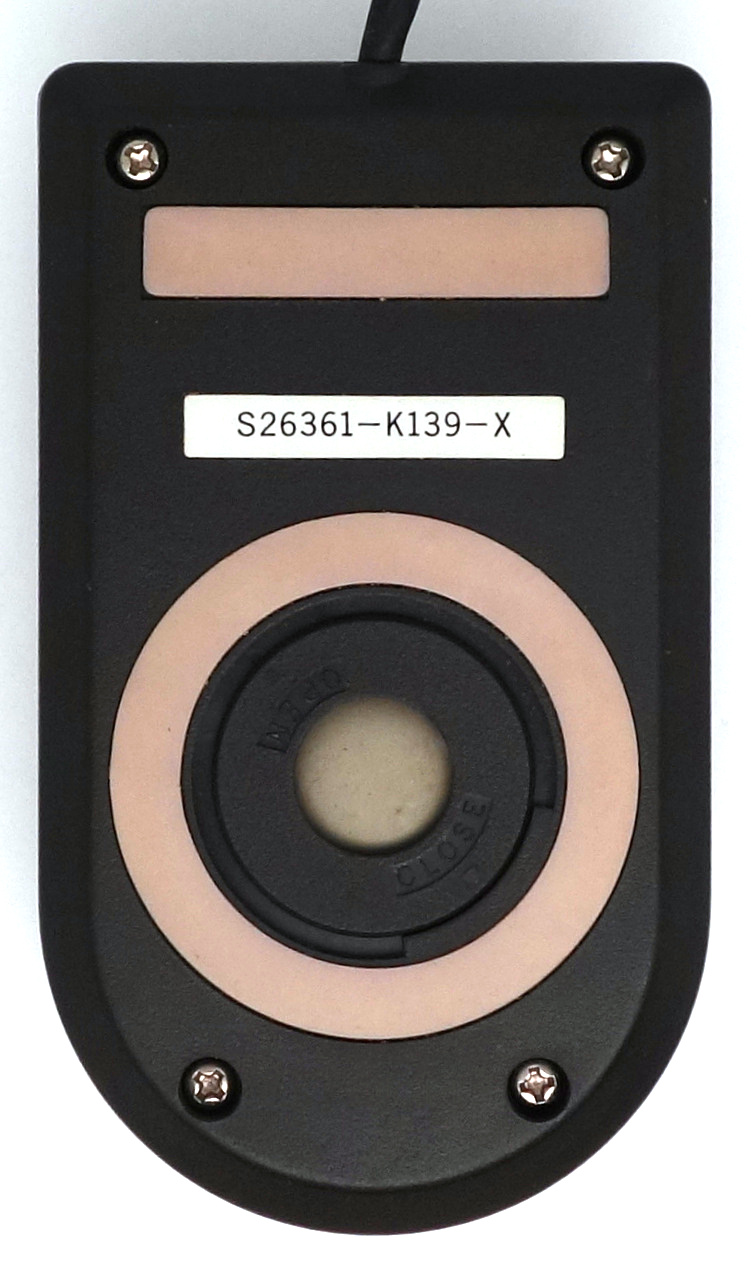
\includegraphics[scale=0.5]{1985_siemens_pcd_mouse/bottom_30.jpg}
    \caption{Siemens PC-D Mouse, top and bottom views}
    \label{fig:SiemensPCDTopBottom}
\end{figure}

In terms of size, the manipulator is an optomechanical cursor control device typical for the 80s (figure \ref{fig:SiemensPCDSize}).

\begin{figure}[h]
    \centering
    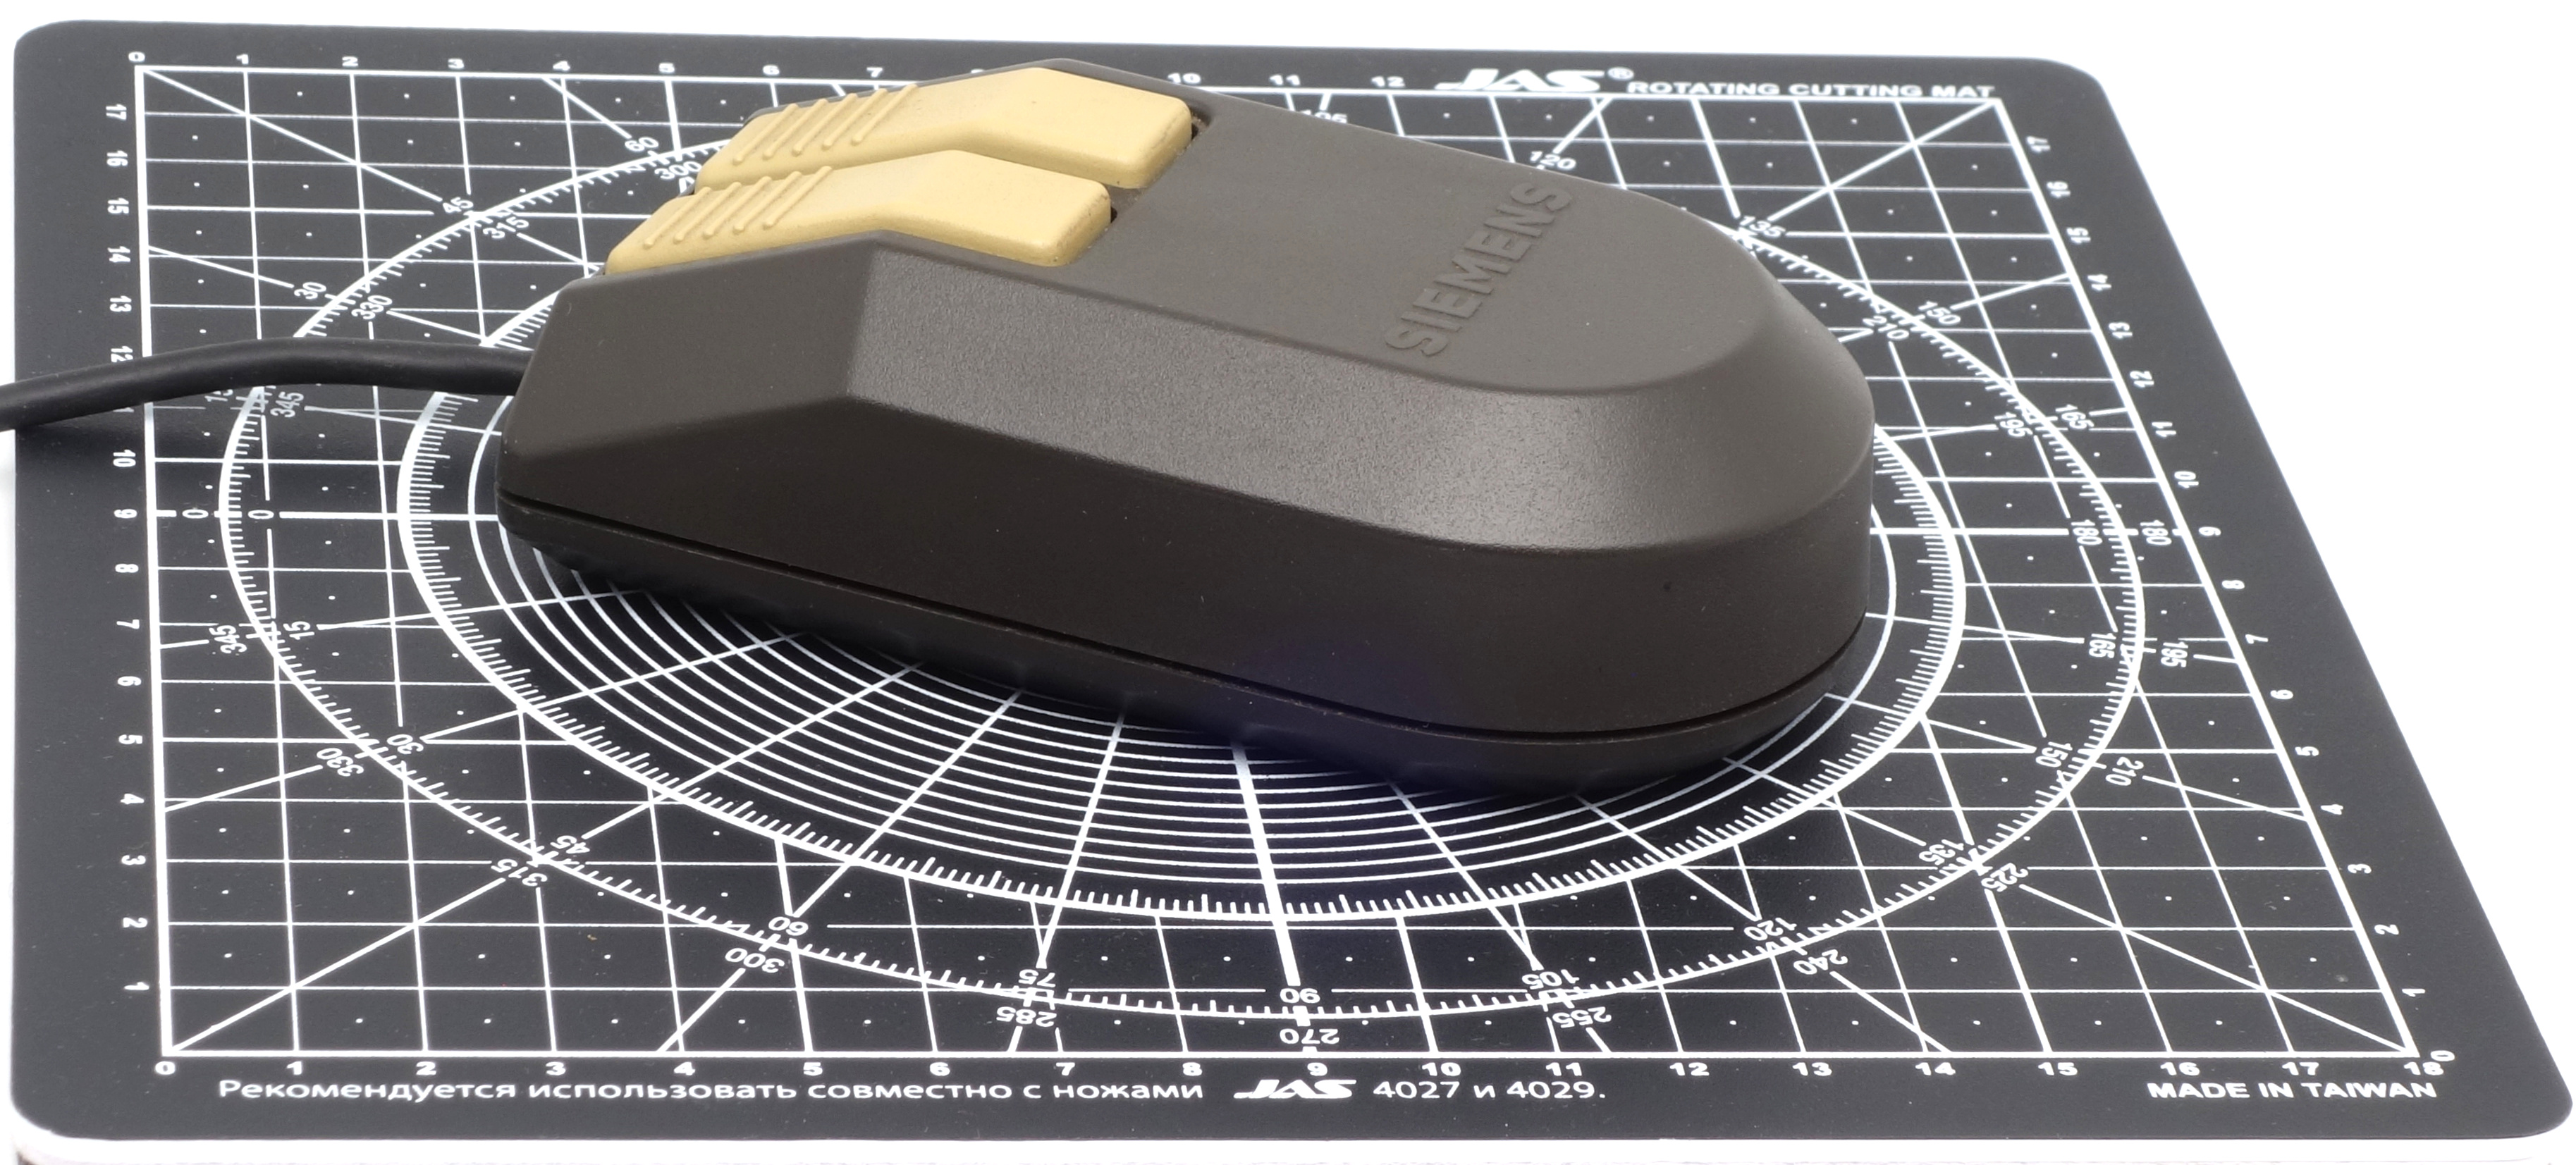
\includegraphics[scale=0.45]{1985_siemens_pcd_mouse/size_30.jpg}
    \caption{Siemens PC-D Mouse on a graduated pad with a grid step of 1~cm}
    \label{fig:SiemensPCDSize}
\end{figure}

In terms of ergonomics, the exterior of PC-D Mouse has a strong industrial design. At the same time, a large number of corners and flat edges are partly compensated by rounded joints of the edges. The buttons are located on the sloping front face and extend onto the upper wall of the body (Fig. \ref{fig:SiemensPCDHand}). According to the manufacturer's recommendation, they should be pressed with the middle and ring fingers, holding the mouse on the sides with the index finger and little finger \cite{manual}.

\begin{figure}[h]
    \centering
    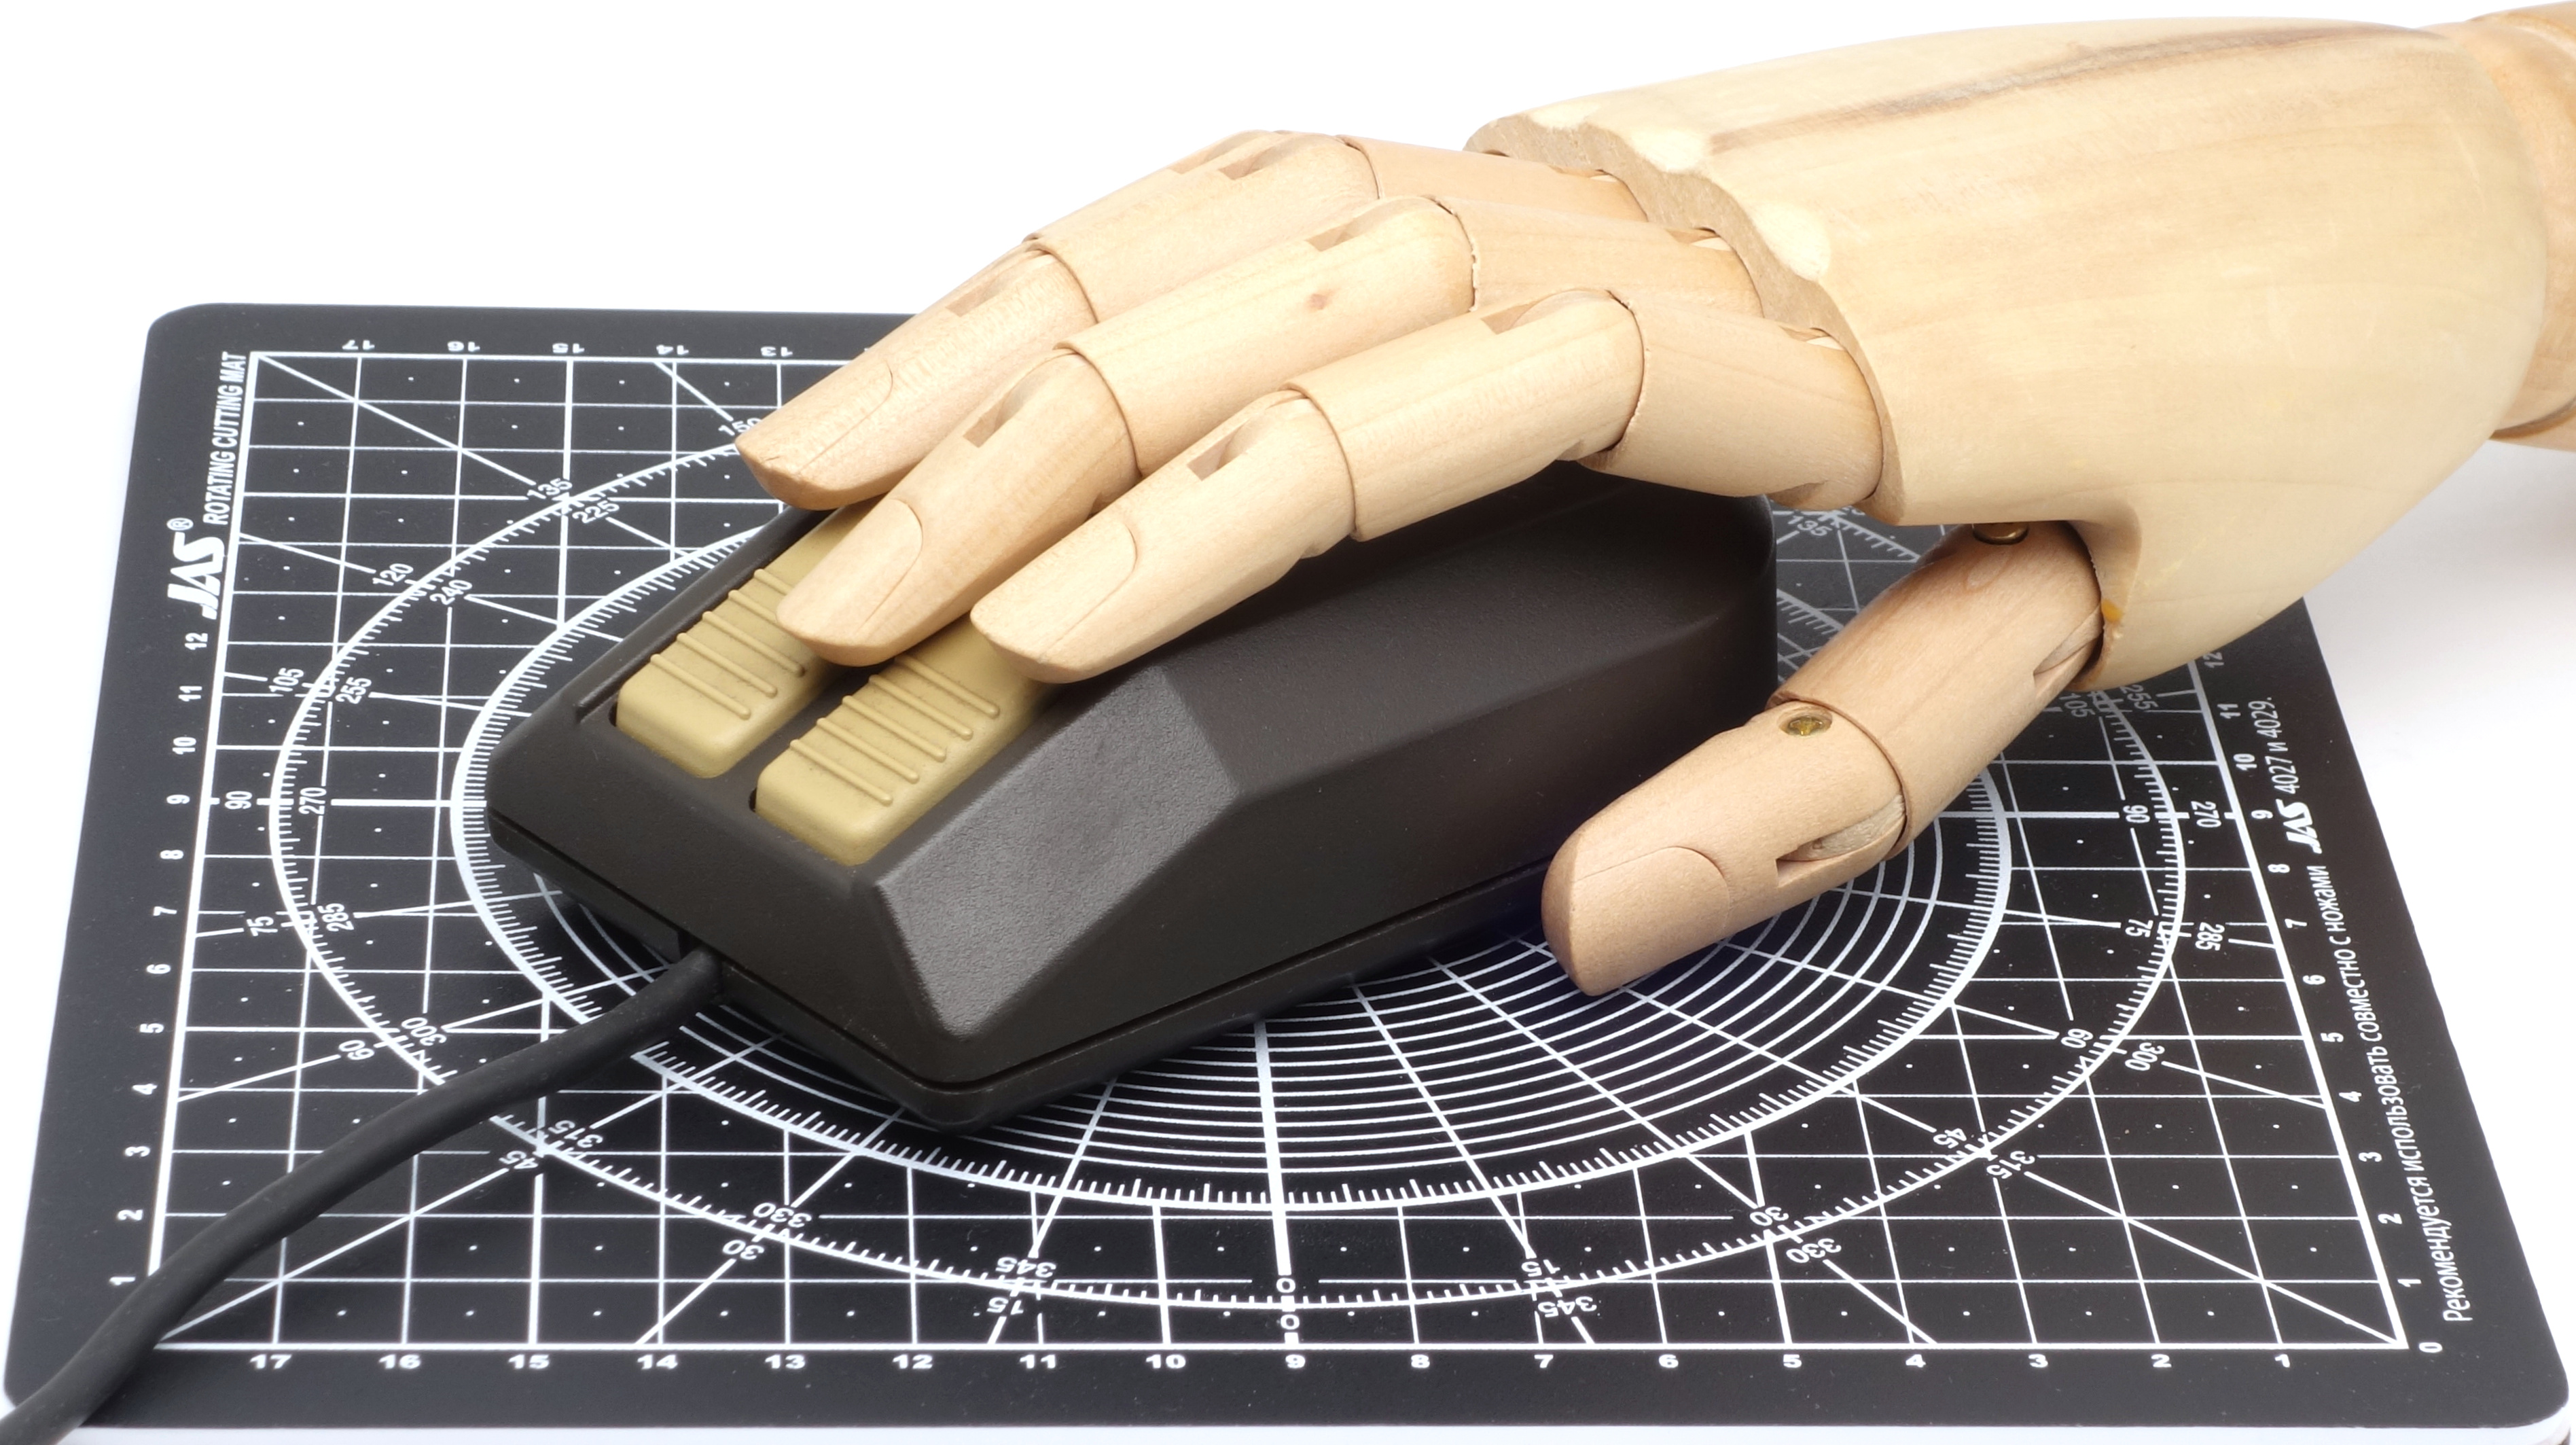
\includegraphics[scale=0.45]{1985_siemens_pcd_mouse/hand_30.jpg}
    \caption{Siemens PC-D Mouse with a human hand model}
    \label{fig:SiemensPCDHand}
\end{figure}

Siemens PC-D Mouse internals are shown on figure \ref{fig:SiemensPCDInside}. The mouse is a device with an opto-mechanical encoder made in Japan.

\begin{figure}[h]
    \centering
    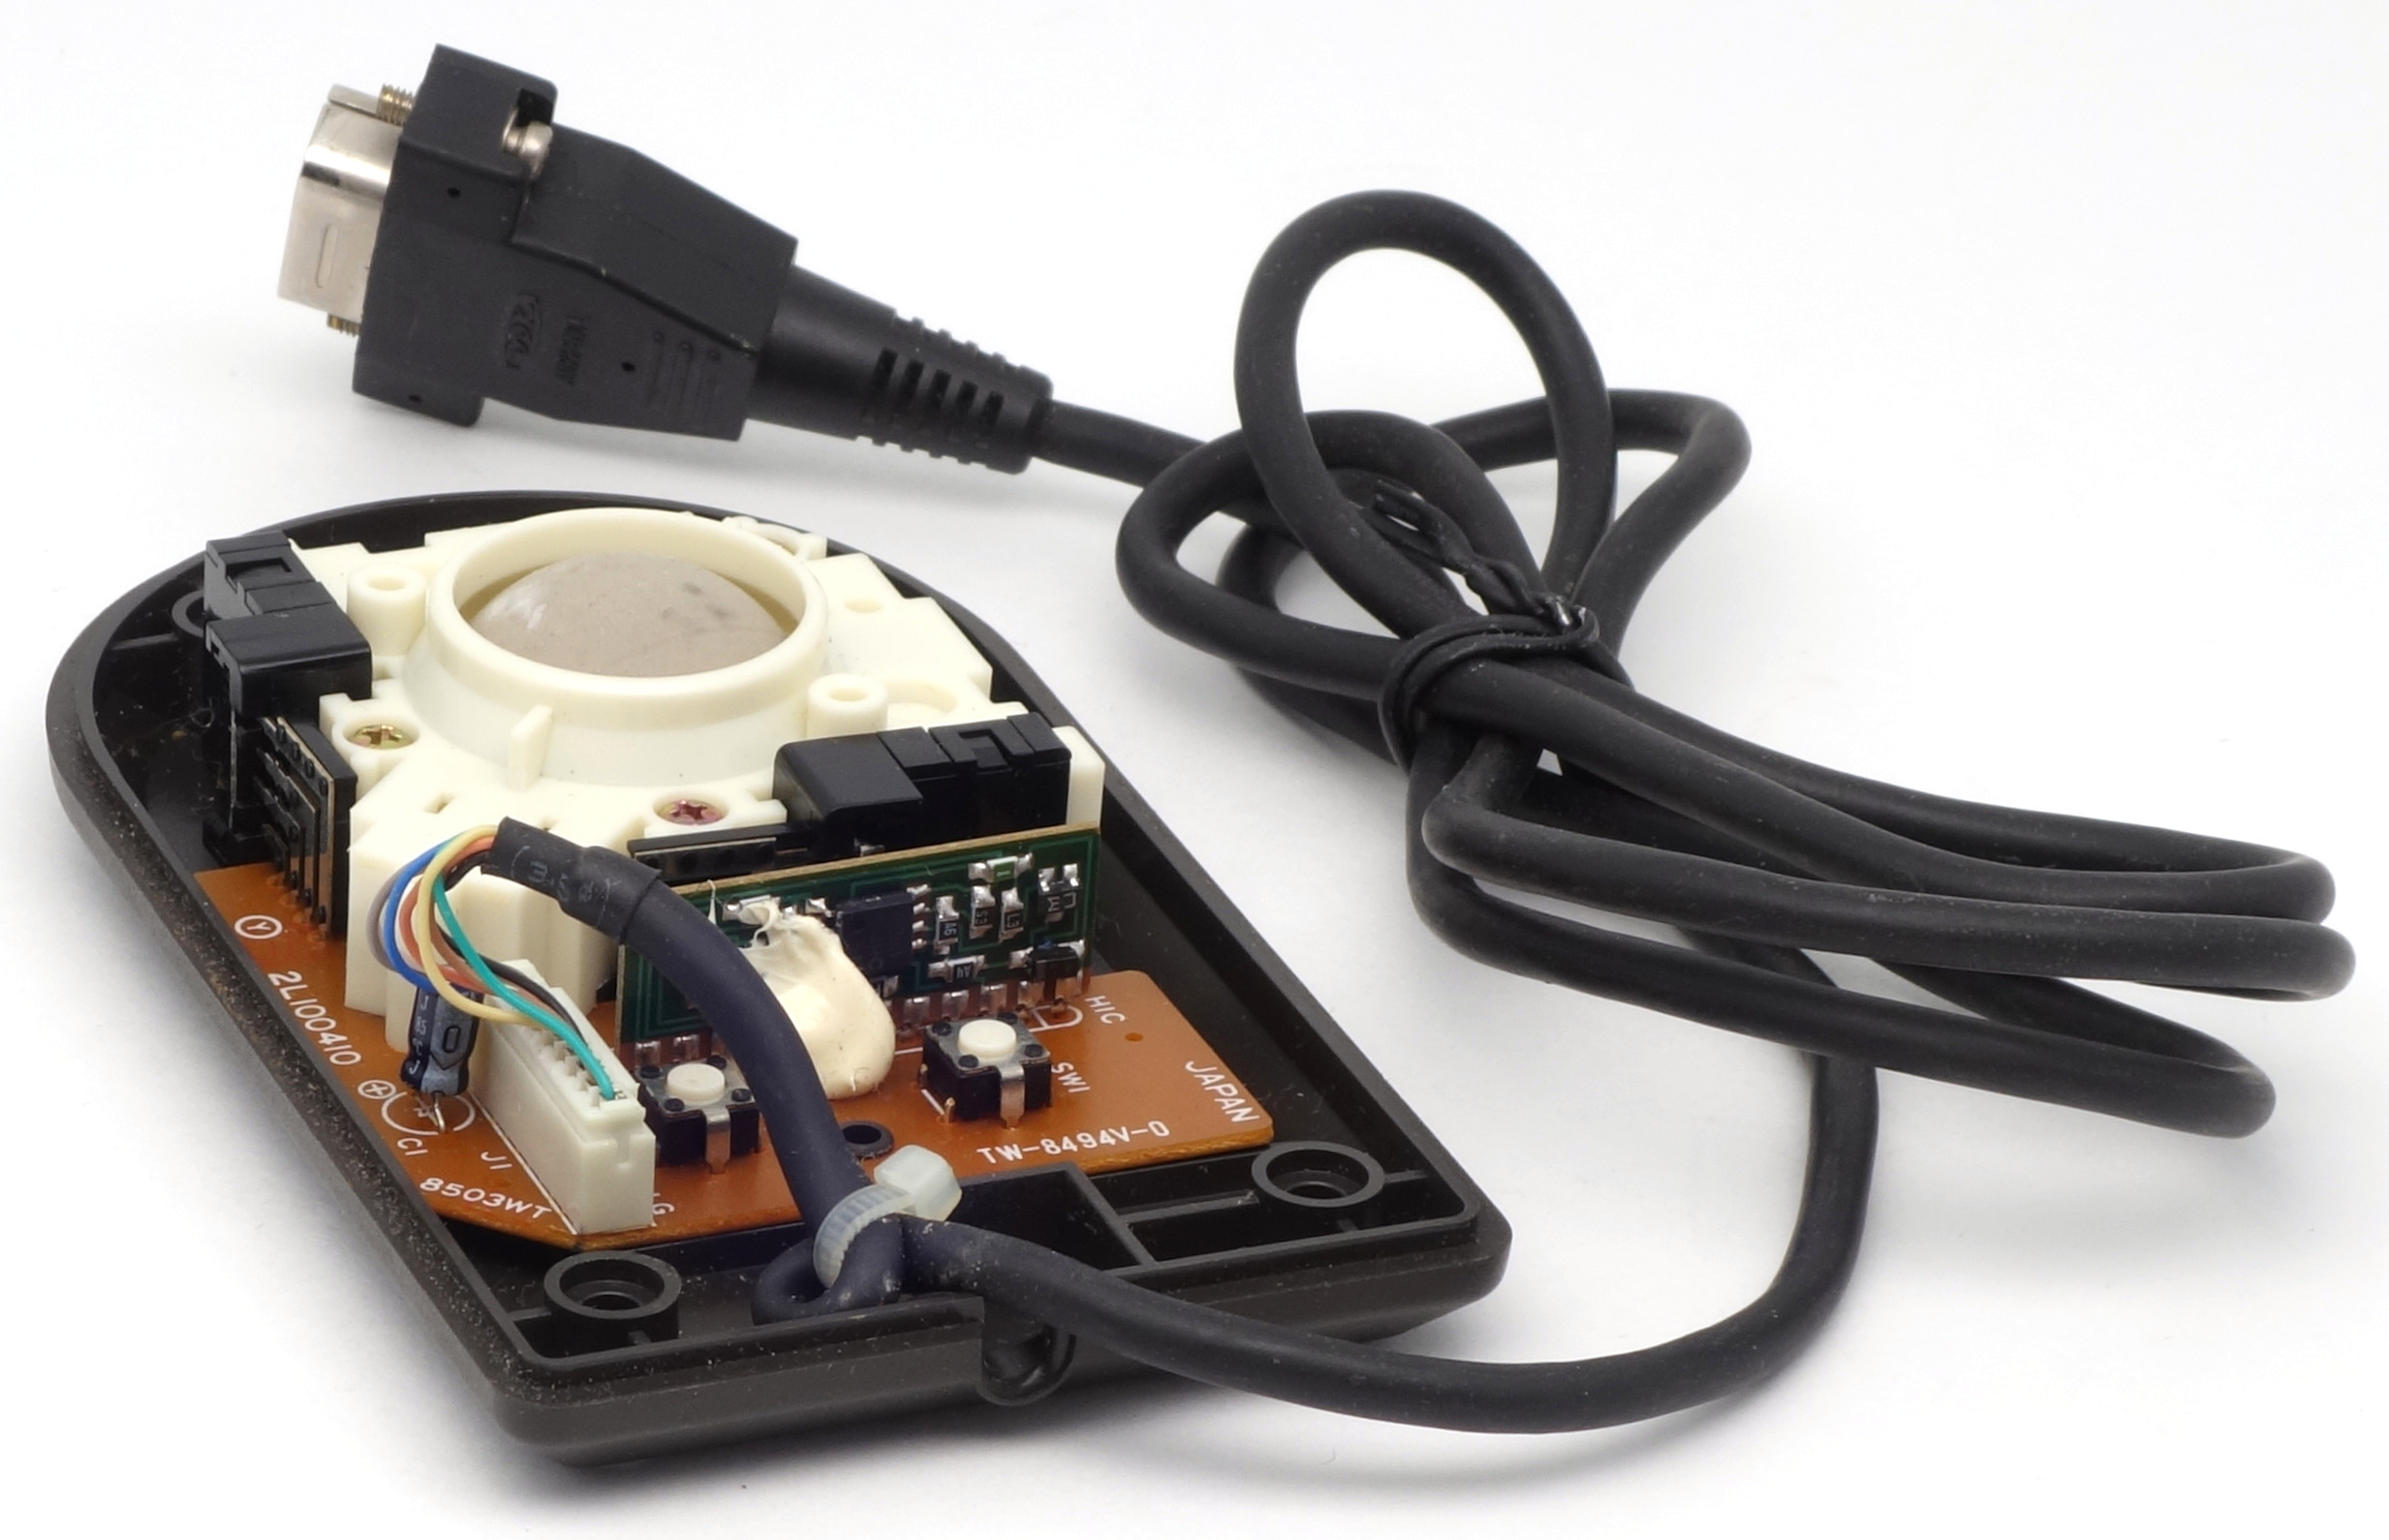
\includegraphics[scale=0.8]{1985_siemens_pcd_mouse/inside_30.jpg}
    \caption{Siemens PC-D Mouse disassembled}
    \label{fig:SiemensPCDInside}
\end{figure}

Apparently, the real manufacturer of the mouse was the Japanese company Alps, which often acted as a contractor in the development of mice for other companies (examples of such companies are IBM, Microsoft, NeXT, Intergraph). Alps usually designed mouse with a unique body shape and buttons layout for each customer, but used the same implementation for several devices. In particular, this mouse has identical parts (the lower part of the body, an optomechanical conversion unit based on closed encoders, a printed circuit board with electronic components) with the original mouse of NeXT computers produced since 1988, and with the mouse of Intergraph InterPro 2020 computers, which appeared on the market in 1992.

\begin{thebibliography}{9}
\bibitem {wiki} Siemens PC-D -- Wikipedia \url{https://en.wikipedia.org/wiki/Siemens_PC-D}
\bibitem {blog} Der PC von Siemens. Heinz Nixdorf MuseumsForum \url{https://blog.hnf.de/der-pc-von-siemens/}
\bibitem {manual} MAUS. Bedienelement für Siemens PC-D. Anwendungsbeschreibung. Ausgabe Dezember 1985. \url{https://github.com/fiowro/mouses/blob/main/source/OCR/PC-D_mouse.pdf}
\end{thebibliography}
\end{document}
